
\chapter{Aprendizaje Automático}
\label{chap:Aprendizaje-Automatico}

\section{Introducción}
En el contexto de aprendizaje automático, los patrones deben ser descubiertos a partir de una serie de muestras que son denominadas instancias. El conjunto de entrada se denomina conjunto de entrenamiento. En nuestro caso específico, cada instancia es un vector de características extraída de señales en una determinada ventana de tiempo. Las muestras en el conjunto de entrenamiento pueden o no ser etiquetadas, es decir, tener asociada a una clase conocida (por ejemplo, caminar, correr, etc.). En algunos casos, tener datos etiquetados no es factible, ya que puede requerir un experto para examinar manualmente los ejemplos y asignar una etiqueta en base a su experiencia.

Este proceso es generalmente tedioso, caro y consume mucho tiempo en muchas aplicaciones de minería de datos. Existen dos enfoques de aprendizaje, es decir, aprendizaje supervisado y no supervisado, que se ocupan de datos etiquetados y no etiquetados, respectivamente. Puesto que un sistema de reconocimiento de la actividad humana debe devolver un resultado como caminar, sentarse, correr, etc., la mayoría de los sistemas de \abbr{HAR} utilizan algoritmos de aprendizaje supervisados. De hecho, podría ser muy difícil de discriminar actividades en un contexto completamente sin supervisión. Algunos otros sistemas funcionan de una manera semisupervisada en donde parte de los datos están sin etiqueta.

\section{Aprendizaje supervisado}
\label{sec3:aprendizaje}De manera a establecer un marco teórico para los algoritmos de aprendizaje automático supervisados \cite{Rajaraman2011} se incluye la siguiente definición formal.

\label{def3:clasificacion}\newtheorem{defs}{Definición}
\begin{defs}(Clasificador\abbr{ML}) Un algoritmo\abbr{ML} recibe un conjunto entrenamiento se compone de varios pares $(\boldsymbol{x},y)$ conocidos como instancias de entrenamiento, donde
\begin{itemize}
\item $\boldsymbol{x}$ es un\emph{vector} de valores, llamado vector característico.
\item $y$ es la\emph{etiqueta}, el valor de clasificación para $\boldsymbol{x}$.
\end{itemize}
El objetivo del proceso\abbr{ML} es encontrar una función $y=f(\boldsymbol{x})$ cuya predicción de $y$ asociada a valores desconocidos de $\boldsymbol{x}$ sea la mejor. El valor de y corresponden a valores arbitrarios pero es común encontrase con los siguientes casos:
\begin{enumerate}
\item $y$ es un número del conjunto de los reales. Este caso corresponde a un problema de regresión.
\item $y$ es un valor booleano verdadero-falso, también representado como $+1$ y $-1$. Este caso corresponde a una clasificación binaria. 
\item $y$ es miembro de un conjunto finito donde cada valor representa una clase particular. El problema es llamado de clasificación de múltiples clases.
\end{enumerate}
\end{defs}

El aprendizaje supervisado, comúnmente conocido como clasificación de múltiples clases discretas, ha sido un campo muy productivo que da lugar a un gran número de algoritmos. En la \tabref{tab3:clasificadores} se resumen los clasificadores más importantes en el estudio de las \abbr{HAR} según su tipo.
\begin{table}
\begin{centering}
\begin{tabular}{|l|l|}
\hline 
		Tipo 						& Clasificador							\\
\hline 
\hline 
		Arboles de Decisión 		& C4.5, ID3								\\
\hline 
		Clasificadores de Bayes 	& Redes de Bayes, \emph{Naïve} Bayes	\\
\hline 
		Basados en Instancia 		& k-vecinos proximos					\\
\hline 
		Transformación de dominio 	& Máquinas de soporte-vector			\\
\hline 
		Redes neuronales 			& Perceptron de múltiples capas			\\
\hline 
		Modelos de Markov 			& Modelos ocultos de Markov				\\
\hline
\end{tabular}
\par\end{centering}
\caption[Algoritmos de \abbr{ML}]{\label{tab3:clasificadores} Algoritmos de aprendizaje automático}
\end{table}

En las siguientes secciones nos concentramos en un enfoque basado en arboles de decisión (\abbr{DT}) para construir la función $f$. La función $f$ corresponde a un árbol de múltiples niveles donde cada nodo aplica una función a $\boldsymbol{x}$ y determina sobre qué nodo hijo procede la búsqueda. Cada nodo posee cualquier número de nodos hijos. Los árboles de decisión son preferibles para las clasificación binaria o de múltiples clases, especialmente cuando la dimensión del vector característicos no es muy grande \cite{Rajaraman2011}.

\section{Arboles de Decisión}
El árbol de decisión es un método de aprendizaje predictivo de una conjunto de tuplas o instancias etiquetadas. Un árbol de decisión es una estructura de árbol similar a un diagrama de flujo, donde cada nodo interno (nodo no hoja) denota una prueba de un atributo, y cada rama representa el camino de a seguir luego de la evaluación, y cada nodo hoja es una etiqueta o clase.

\begin{figure}[!htbp]
	\centering
	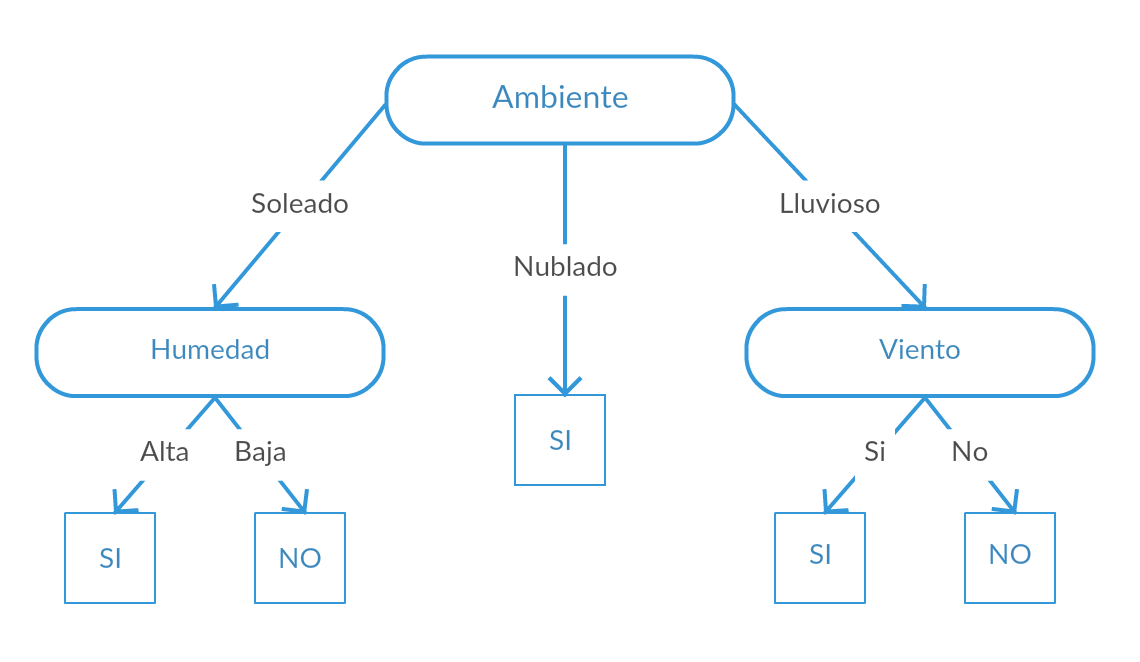
\includegraphics[width=0.7\linewidth]{capitulo-3/graphics/ad_2}
	\caption[Árbol de decisión]{Árbol de decisión}
	\label{fig:arbolEjemplo}
\end{figure}

En la figura por ejemplo un típico árbol de decisión que representa el concepto de jugar o no Golf, teniendo en cuenta variables climática representadas en los nodos internos, y los nodos hojas denotan las decisiones de jugar o no golf. 

\section{Algoritmo C4.5}
J.R Quinlan propone un mejora, una extensión al algoritmo ID3, al que denomina C4.5, este algoritmo genera un árbol de decisión a partir de los datos mediante particiones realizadas recursivamente. El árbol se construye mediante la estrategia profundidad-primero (\emph{depth-first}).

El algoritmo C4.5 utiliza técnica heurística conocida como proporción de ganancia (\emph{gain-ratio}). Es una medida basada en información que considera diferentes números y probabilidades de los resultados de las pruebas. 

El algoritmo considera todas las pruebas posibles que puede dividir el conjunto de datos, seleccionar la prueba que le haya generado mayor ganancia de información. Para cada atributo discreto, se considera una prueba con $N$ resultados, siendo $N$ el numero de valores posibles que puede tomar el atributo. Para cada atributo continuo, se realiza la prueba binaria (1,0) sobre cada uno de los valores que puede tomar el atributo de los datos.

\section{Características del algoritmo C4.5}
\begin{itemize}
	\item Permite trabaja con valores continuos para los atributos, separando los posibles resultados en dos ramas $ A_{i} <= N $ y $ A_{i} > N $ . 
	\item Los arboles son menos frondosos, ya que cada hoja cubre una distribución de clases no una clase en particular.
	\item Utiliza el método 'divide y vencerás' para generar el árbol de decisión inicial a partir de un conjunto de datos de entrenamiento.
	\item Se basan en la utilización del criterio de proporción de ganancia, definido como $ I(X_{i},C) / I(X_{i})  $. De esta manera se consigue evitar que la variables con mayor numero de categorías salgan beneficiadas en la selección. 
	\item Es recursivo.
\end{itemize}

\section{Información de Ganancia / Entropía }
C4.5 como su predecesor ID3 utiliza la entropía como medida de selección para el atributo. 
Dado un nodo $N$ que representa las tuplas de la partición $D$. El atributo con mayor valor de ganancia es elegido para la división de $N$, el atributo reduce al mínimo la información necesaria para clasificar las tuplas de las particiones resultantes y refleja la menos aleatoriedad o impureza de la partición. Este enfoque minimiza el número esperado de los ensayos necesarios para clasificar una tupla dada y garantiza que un árbol simple (pero no necesariamente el más simple) se encuentre.

La información de ganancia necesaria para clasificar una tupla en $D$ es igual a:

\begin{equation}
Info(D) = - \displaystyle\sum_{i=1}^{m} p_{i}\log_2(p_{i}) 
\end{equation}

donde $p_{i}$ es la probabilidad de una tupla arbitraria en $D$ que pertenece a la clase $C_{i}$ se estima que es $ \lvert C_{i,D}} \rvert / \lvert D \rvert $. Se utiliza un logaritmo en base 2 porque la información esta codificada en bits. $Info(D)$ es la cantidad media de información necesaria para identificar la etiqueta de una tupla dada en $D$. Nótese, que la información que tenemos se basa solamente en las proporciones de tuplas de cada clase. $Info(D)$ también se conoce como entropía de $D$

Ahora, supongamos que estábamos para particionar las tuplas en $D$ en algunos atribuyen A teniendo $v$ valores distintos $ \{ a_{1},a_{2},...,a_{v} \}$, como se observa a partir de los datos de entrenamiento. Si A tiene valores discretos, estos valores se corresponden directamente con los resultados de una prueba de $v$ sobre $A$. El atributo $A$ se puede utilizar para dividir $D$ en $v$ particiones o subconjuntos, $ \{ D_{1},D_{2},...,D_{v} \}$, donde $D_j$ contiene aquellas tuplas en $D$ que tienen $a_j$ resultados de $A$. Estas particiones se corresponderían con las ramas que crecen a partir del nodo $N$. Idealmente, nos gustaría que esta división para producir una clasificación exacta de las tuplas. Es decir, nos gustaría para cada partición sea pura. Sin embargo, es bastante probable que las particiones sea impura (por ejemplo, cuando una partición puede contener una colección de tuplas de diferentes clases en lugar de una sola clase). ¿Cuánto más información sería todavía necesaria (después de la partición) con el fin de llegar a una clasificación exacta? Esta cantidad se mide por:

\begin{equation}
Info_{A}(D) = \displaystyle\sum_{j=1}^{v} \displaystyle\frac{\lvert D_{j} \rvert}{\lvert D \rvert} \times Info(D_{j})
\end{equation}

El termino $\displaystyle\frac{\lvert D_{j} \rvert}{\lvert D \rvert}$ actúa como el peso de la j-esima partición. $Info_{A}(D)$ es la información esperada requerida para clasificar la tupla de $D$ basada en la partición de $A$. Cuando menor sea la información esperada, mayor es la pureza de las particiones.

La información de ganancia se define como la diferencia entre lo requerido de información original (basado en la proporción de clases) y el nuevo requerimiento, obtenido luego de realizar la partición en $A$. Es decir,

\begin{equation}
Gain(A) = Info(D) - Info_{A}(D).
\end{equation}

En otras palabras, $Gain(A)$ nos dice cuanto se ganaría por la ramificación en $A$. Es la reducción esperada en el requisito de información causado por conocer el valor de $A$. El atributo A con ganancia mas alta, $Gain(A)$, se selecciona como atributo de división en el nodo $N$. Esto equivale a decir que queremos particionar en el atributo A que haría la mejor clasificación, por lo que la cantidad de información aun necesaria para clasificar las tuplas sea minima, $InfoA(D)$.


\section{Algoritmo}

\begin{algorithm}
	\caption{Árbol de Decisión - C4.5}
	\label{algoC45}
	\begin{algorithmic}[1]
		\Require Conjunto de datos etiquetados $D$
		\Procedure{C4.5}{$ D $}
			\If {$D > \textit{es puro o cumple el criterio de parada} $} 
				\State\textit{Termina}
			\EndIf
			\ForAll{$a \in D $}
				\State $\textit{Computar información de division en a }$
			\EndFor
			\State $ a_{best} =$ Mejor atributo de división respecto al criterio 
			\State $ Arbol =$ Crear un nodo de decisión con $ a_{best} $ en la raíz 
			\State $ D_{v} =$ Introducir sub-conjunto de $D$ basado en división $ a_{best} $
			\ForAll{$ D_{v} $}
				\State $ Arbol_{v} = C4.5(D_{v}) $
				\State Unir $ Arbol_{v} $ al correspondiente arco del Árbol
			\EndFor
			\State 
			\Return $ Arbol $
		\EndProcedure
	\end{algorithmic}
\end{algorithm}

\section{Ejemplo 1}

En la siguiente tabla se presenta un conjunto de entrenamiento $D$, con la clase etiquetada, de una base de datos de compra de productos electrónicos. En este ejemplo, cada atributo tiene un valor discreto, los atributos de valores continuos fueron generalizados. La clase \textit{Compra Computador} tiene dos valores posible {Si, No}, por lo tanto dos clases distintas (es decir, $m=2$). Tenemos $C_1$ que corresponde a $Si$ y $C_2$ corresponde a $No$.
Existen nueve tuplas de la clase "Si", y cinco de la clase "No". Para encontrar el criterio de división para las tuplas debemos calcular la ganancia de información de cada atributo. Primero usamos la ecuación 3.1 para calcular esperada necesaria para clasificar una tupla en $D$:

\begin{equation*}
Info(D) = - \frac{9}{14}\log_2(\frac{9}{14}) - \frac{5}{14}\log_2(\frac{5}{14})	= 0.940 bits
\end{equation*}

\begin{table}[htbp]
	\caption{Ejemplo de conjunto de entrenamiento}
	\label{tabla:sencilla2}
	\begin{tabular}{|c|l|l|l|l|c|}
		\hline 
		\textbf{Rid} & \textbf{Edad}    & \textbf{Ingreso} & \textbf{Estudiante} & \textbf{Rating Crediticio} & \textbf{Compra Computador?} \\
		\hline 
		\hline
		1   & Joven   & Alto    & No         & Justa             & NO                 \\ 
		2   & Joven   & Alto    & No         & Excelente         & NO                 \\ 
		3   & Mediana & Alto    & No         & Justa             & SI                 \\ 
		4   & Adulto  & Medio   & No         & Justa             & SI                 \\ 
		5   & Adulto  & Bajo    & Si         & Justa             & SI                 \\ 
		6   & Adulto  & Bajo    & Si         & Excelente         & NO                 \\ 
		7   & Mediana & Bajo    & Si         & Excelente         & SI                 \\ 
		8   & Joven   & Medio   & No         & Justa             & NO                 \\ 
		9   & Joven   & Bajo    & Yes        & Justa             & SI                 \\ 
		10  & Adulto  & Medio   & Si         & Justa             & SI                 \\
		11  & Joven   & Medio   & Si         & Excelente         & SI                 \\
		12  & Mediana & Medio   & No         & Excelente         & SI                 \\
		13  & Mediana & Alto    & Si         & Justa             & SI                 \\
		14  & Adulto  & Medio   & No         & Excelente         & NO                 \\
		\hline
		\hline
	\end{tabular}
\end{table}

Luego, necesitamos calcular la información requerida por cada atributo. Comenzamos con el atributo $Edad$, necesitamos observar la distribución de $Si$ y $No$ por cada categoría o valor del atributo $Edad$. Para la categoría $Joven$ de edad, hay dos tuplas $Si$ y tres tuplas $No$. Para la categoría $mediana$ edad, hay cuatro tuplas $Si$ y cero tuplas $No$. Para la categoría $Adulto$, hay tres tuplas $Si$ y dos tuplas $No$. Usando la ecuación (3.2), la información esperada necesaria para clasificar una tupla en $D$ si las tuplas son divididas según el atributo $edad$:

\begin{equation*}
\begin{split}
Info_{edad}(D) & = \frac{5}{14} \times ( -\frac{2}{5}\log_2(\frac{2}{5})-\frac{3}{5}\log_2(\frac{3}{5})  ) \\
			   & + \frac{4}{14} \times ( -\frac{4}{4}\log_2(\frac{4}{4})-\frac{0}{4}\log_2(\frac{0}{4})  ) \\
			   & + \frac{5}{14} \times ( -\frac{3}{5}\log_2(\frac{3}{5})-\frac{2}{5}\log_2(\frac{2}{5})  ) \\
			   & = 0.694 bits.
\end{split}
\end{equation*}

Por lo tanto, la ganancia esperada de realizar tal partición seria:

\begin{equation*}
Gain(edad) = Info(D) - Info_{edad}(D) = 0.940 - 0.694 = 0.246 bits
\end{equation*}

De la misma manera, se puede calcular $Gain(ingreso)$ = 0.029 bits, $Gain(estudiante)$ = 0.151 bits, y $Gain(RatingCrediticio)$ = 0.048 bits. Debido a que el atributo $edad$ tiene mayor ganancia de información, es seleccionado para realizar la partición. El nodo $N$ es etiquetado con $edad$, y se crean una rama por cada valor del atributo. Las tuplas se divinen en consecuencia, como se muestra en la figura . Notese que las tuplas en la partición $Edad = Mediana$ perteneces todas a la clase $Si$, por lo tanto en esta rama se crea una hoja con etiqueta $Si$. El árbol de decisión final devuelto por el algoritmo se muestra en la figura \ref{fig:arbolEjemplo}.

\begin{figure}[!htbp]
	\centering
	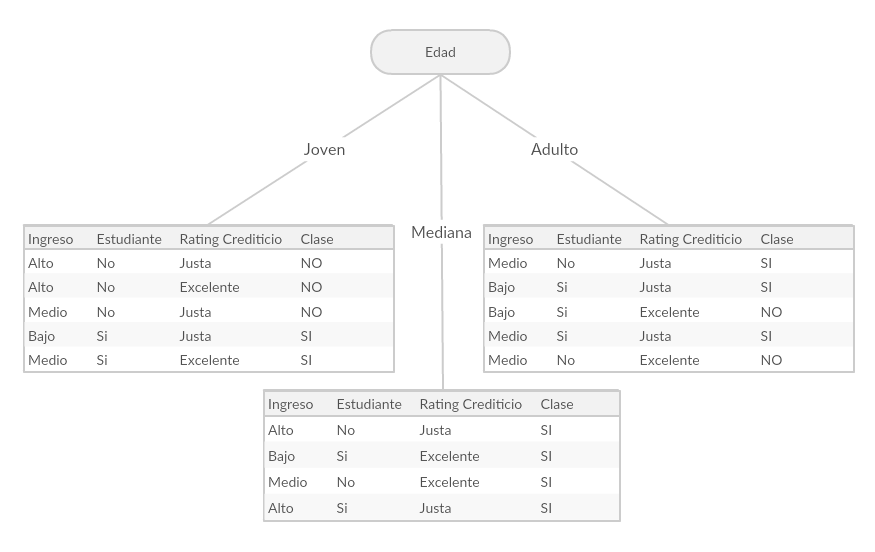
\includegraphics[width=0.7\linewidth]{capitulo-3/graphics/dtree_parti}
	\caption[Árbol de decisión]{Árbol de decisión: Particionado en el atributo 'Edad'}
	\label{fig:arbolPartEdad}
\end{figure}

\section{Métricas de evaluación y Matriz de Confusión}
En general, la selección del algoritmos de clasificación para HAR ha sido apoyada meramente por evidencias empíricas. La gran mayoría de los estudios utilizar una validación cruzada con pruebas estadísticas para comparar el rendimiento de los clasificadores para un conjunto de datos determinado, como se visualiza en la \ref{fig:evaluacion}.

\begin{figure}[!htbp]
	\centering
	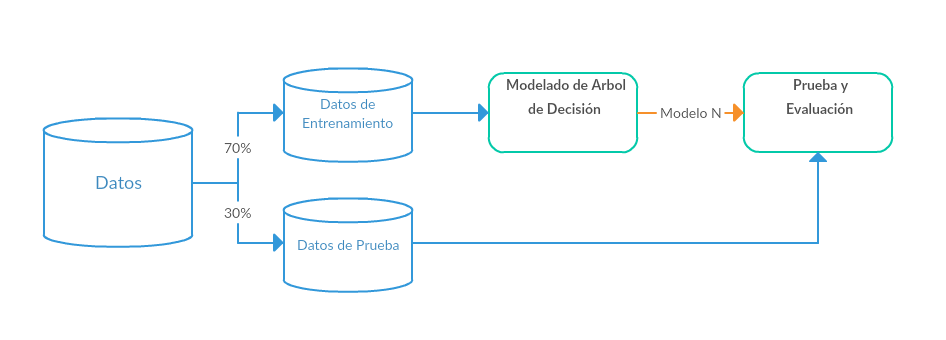
\includegraphics[width=0.7\linewidth]{capitulo-3/graphics/training-test}
	\caption[Diagrama de Evaluación de Clasificación]{Diagrama de Evaluación de Clasificación}
	\label{fig:evaluacion}
\end{figure}
	
Los resultados de una clasificación de un métodos en particular se suelen organizar en una matriz de confusión $M_{n \times n}$ para un problema de  clasificación con $N$ clases.
Esta es una matriz, tal que el elemento $M_{ij}$ es el numero instancias de la clase $i$ que realmente fueron clasificados como clase $j$.
Los siguientes valores se pueden obtener de la matriz de confusión en un problema de clasificación primaria:

\begin{itemize}
	\item Verdaderos Positivo (TP): El número de casos positivos que fueron clasificados como positivos.
	\item Verdaderos Negativo (TN): El número de casos negativos que fueron clasificados como negativos.
	\item Falso Positivo (FP): El número de casos negativos que fueron clasificados como positivos.
	\item Falso Negativo (FN): El número de casos positivos que fueron clasificados como negativos.
\end{itemize}

La precisión es la métrica más estándar para resumir el rendimiento general de la clasificación para todas las clases y se define de la siguiente manera:

\begin{equation}
Exactitud = \frac{TP + TN}{TP + TN + FP + FN}
\end{equation}

La precisión, a menudo denominada valor predictivo positivo, es la proporción de casos positivos clasificados correctamente al número total de casos clasificados como positivos:
\begin{equation}
\mbox{Precisión} = \frac{TP}{TP + FP}
\end{equation}

La exhaustividad, también llamado tasa positiva verdadera, es la proporción de instancias positivas correctamente clasificadas al número total de instancias positivas:
\begin{equation}
Exhaustividad = \frac{TP}{TP + FN}
\end{equation}


El Valor-F combina precisión y exhaustividad en un solo valor:
\begin{equation}
Valor-F = 2 \cdot \frac{\mbox{Precisión} \cdot Exhaustividad}{\mbox{Precisión} + Exhaustividad}
\end{equation}

Aunque se definen para la clasificación binaria, estas métricas pueden generalizarse para un problema con n clases. En tal caso, una instancia podría ser positiva o negativa según una clase particular, por ejemplo, los positivos podrían ser todas las instancias de ejecución mientras que los negativos serían todas las instancias distintas de la ejecución.

\section{Ejemplo: Evaluación}

Utilizando el ejemplo anterior en la tabla \ref{tabla:sencilla2}, se tomo una muestra de 10.000 tuplas, teniendo como resultado la tabla \ref{tabla:MatrizConfusion}


\begin{table}[htbp]
	\caption{Matriz de Confusión}
	\label{tabla:MatrizConfusion}
	\begin{tabular}{|l|c|c|c|}
		\hline 
		\textit{Clase} & \textit{Com. Computador = SI}    &\textit{Com. Computador = NO} & \textit{Total}  \\
		\hline 
		\textit{Com. Computador = SI}	& 6,954   	& 46    	& 7,000     \\ 
		\textit{Com. Computador = NO}	& 412		& 2,588		& 3,000    	\\ 
		\hline
		\textit{Total}					& 7,366		& 2,634    	& 10,000	\\ 
		\hline
	\end{tabular}
\end{table}


Tomando este ejemplo, para la clase \textit{Compra Computador = SI} tenemos lo siguiente:

\begin{itemize}
	\item Verdaderos Positivo (TP): 6,954
	\item Verdaderos Negativo (TN): 2,588
	\item Falso Positivo (FP): 412
	\item Falso Negativo (FN): 46
\end{itemize}

Con estos datos podemos calcular el resto de las métricas:
\begin{equation*}
Exactitud = \frac{TP + TN}{TP + TN + FP + FN} = \frac{6,954 + 2,588}{6,954 + 2,588 + 412 + 46} = \frac{9542}{10000} = 0,9542
\end{equation*}

\begin{equation*}
\mbox{Precisión} = \frac{TP}{TP + FP} = \frac{6,954}{6,954 + 412} = 0,9440
\end{equation*}

\begin{equation*}
Exhaustividad = \frac{TP}{TP + FN} = \frac{6,954}{6,954 + 46} = 0,9934
\end{equation*}

\begin{equation*}
Valor-F = 2 \cdot \frac{\mbox{Precisión} \cdot Exhaustividad}{\mbox{Precisión} + Exhaustividad} 
		= 2 \cdot \frac{\mbox{0,9440} \cdot 0,9934}{\mbox{0,9440} + 0,9934}
		= 0,4840
\end{equation*}

